\documentclass[pageno]{jpaper}
%\newcommand{\iscasubmissionnumber}{117}

\usepackage[normalem]{ulem}
\usepackage{booktabs}
\usepackage{mathtools}
\usepackage{ragged2e}
\usepackage{rotating}
\usepackage{array}
\usepackage{grffile}

\usepackage{epsfig}
\usepackage{float}
\usepackage{wrapfig}
\usepackage{setspace}
\usepackage{multirow}
\usepackage{graphicx}
\usepackage{fancyhdr}
%\usepackage{paralist}
%\usepackage{capt-of}

\usepackage{color}
\usepackage{xcolor,colortbl}
\usepackage{chngpage}
\usepackage{enumitem}
\usepackage{enumerate}
\usepackage{amsmath,relsize}
\usepackage[justification=centering]{caption}
\usepackage{tabu}
\usepackage{stmaryrd} % short right arrow

\usepackage{listings}
\usepackage[makeroom]{cancel}


\usepackage{amssymb}% http://ctan.org/pkg/amssymb
\usepackage{pifont}% http://ctan.org/pkg/pifont
\usepackage[nomargin,inline,draft]{fixme}
\newcommand{\cm} {\clap{\small\ding{51}}\small\hphantom{--}}
\newcommand{\cmi}{\clap{\small\ding{51}-}\small\hphantom{--}}%
%\newcommand{\xm} {\clap{\ding{55}}\hphantom{--}}
\newcommand{\xm} {\clap{\small}\small\hphantom{--}}

\newcommand{\Forall}{\displaystyle\mathop\mathlarger{\mathlarger{\mathlarger{\forall}}} } 

%\newcommand{\cm} {{Y}}%
%\newcommand{\cmi}{{P}}%
%\newcommand{\xm} {{}}%


\usepackage{tikz,array}
\usetikzlibrary{calc}

%\newcommand*\circled[1]{\tikz[baseline=(char.base)]{
%            \node[shape=circle,draw,inner sep=2pt] (char) {#1};}}

%\newcommand*\ccircled[1]{\tikz[baseline=(char.base)]{
%            \node[shape=circle,draw,inner sep=2pt] (char) {#1};}}

\tikzstyle{every node}=[font=\footnotesize]

\newcommand{\hcancel}[5]{%
    \tikz[baseline=(tocancel.base)]{
        \node[inner sep=0pt,outer sep=0pt] (tocancel) {#1};
        \draw[black] ($(tocancel.south west)+(#2,#3)$) -- ($(tocancel.north east)+(#4,#5)$);
    }%
}%

\newcommand*\circled[1]{\tikz[baseline=(char.base)]{
            \node[shape=circle,draw,inner sep=0.5pt, minimum size=0.24cm] (char) {#1\vphantom{H}};}}

\newcommand*\ccircled[1]{\hcancel{\tikz[baseline=(char.base)]{
            \node[shape=circle,draw,inner sep=0.4pt, minimum size=0.24cm] (char) {#1\vphantom{H}};}}{-1pt}{1pt}{1pt}{-1pt} }


\begin{document}
\title{
\vspace{-0.15in}
An Efficient GPGPU Implementation of Viola-Jones Classifier Based Face Detection Algorithm
\vspace{-0.15in}
}





\author{Sharmila Shridhar  \\ \and  
    Ramsai Manoj Bamdhamravuri  \\ \and 
        Vinay Gangadhar 	\\ \and
            \{sshridhar, bamdhamravur, gangadhar\}@wisc.edu} 

\date{}
\maketitle

%\thispagestyle{empty}
\begin{abstract}
   
\vspace{0.1in}

Applications with large amount of data level parallelism
can benefit from General Purpose based Graphics Processing
Units (GPGPUs) because of better energy efficiency and performance compared to a CPU. Due to GPGPUs’ impressive
computing throughput and memory bandwidth, many applications with enough parallelism can take advantage of acceleration using GPGPU. Computer vision algorithms are one such
workload domain which can better utilize the large number
of cores in GPU, and hence meet their real-time requirements
of the applications. One such application is \emph{Face Detection}
which has real-time constraint on its execution. Sequential
processing of image windows with image downsampling and classifiers on CPU is difficult to meet the real-time requirements. 

In this project, we have
implemented the face detection acceleration algorithm based
on Viola-Jones cascade classifier on the GPGPU CUDA platform.
We have considered different portions of the viola jones algorithm which include 
\emph{nearest neighbor}, \emph{integral image} and {HAAR classifier} that can
be parallelized.
We identify different bottlenecks in GPU implementation and include optimizations
which gives the performance benefit. We explain each of these optimizations in detail for all the kernels. 
We finally compare the execution of the same algorithm executed
on the CPU and analyze the gains from the GPU.
We achieve a speedup upto 5.35x (including the inclusive time) compared to the single threaded performance of CPU.




\end{abstract}

\section{Introduction}\label{sec:intro}

With recent advances in computing technology, and new computing capabilities
with GPGPU hardware~\cite{owens2008gpu} and programming models~\cite{nvidia2007compute}, 
a trend of mapping many image processing applications on GPU is seen. 
Compute Unified Device Architecture (CUDA) has enabled mapping generic parallel
implementations of image processing algorithms~\cite{yang2008parallel} easier and benefits with good amount of 
performance and energy efficiency. 
Face detection is one such application which has lots of fine-grained
data parallelism available and exploit the execution resources of GPU.
It is processing of taking an image and detecting and locating the faces 
in the given image. It is an important application used world-wide for
public security, airports, video conferencing and video surveillance. 

Most of face detection systems today use cascade classifier algorithm 
based on Viola and Jones~\cite{viola2001rapid}. It has three important 
concepts tied to it -- integral image calculation, Adaboost classifier training
algorithm~\cite{freund1999short} and cascade classifier.  
Although, many of them have implemented these algorithm in CPUs, due to 
the inherent serial nature of CPU execution, you cannot get much of the
performance benefit and may not be able to meet hard real-time constraints,
even when executed on a multi-core CPU. 
With face detection algorithm's inherent parallel characteristics, GPGPU 
parallel computing substrate is a good candidate to gain performance benefits. 
With recent advances in NVIDIA CUDA programming model for scientific application 
acceleration~\cite{buck2007gpu}, we aim to use GPGPU execution model for accelerating face detection algorithm.

In this project, we have implemented the  face detection algorithm 
based on the Viola Jones classifier on GPU. 
As a starting point, we take the GNU licensed C++ program that has the 
algorithm implemented to detect faces in images. We also take the already trained 
classifier network which includes different HAAR classifier features trained based on thousands of images. 
We have identified the different  portions of the algorithm that 
can be parallelized and leverage the execution with abundant GPU resources efficiently. 
We have implemented all the three phases of the face detection -- nearest neighbor, integral image calculation and
scanning window stage along with classifying the output from each classifying stage. 
As a course project we limited the implementation to these 3 stages mentioned above, 
and not focus on the training of classifier itself. We take some insights and principles
based on previous implementations of face detection on GPGPUs, FPGA done here~\cite{kong2010gpu, sun2013acceleration, cho2009fpga}.
The main focus of this project was to gain performance benefits out of face detection acceleration and characterize
the bottlenecks if there are any. Based on those principles, we found many bottlenecks in the GPU implementation and add
optimizations to address these bottlenecks. We evaluate our GPU implementation performance with respect to single threaded CPU performance 
and we achieve a speedup upto 5.35x including the GPU inclusive time of copying.

We present the overview of our paper here:
Section \ref{sec:viola} explains the Viola Jones algorithm briefly and Section \ref{sec:impl} explains the our implementation of face detection.
Section \ref{sec:nnii} and Section{sec:haar} explain the three parallel versions of the algorithm we have implemented. Section\ref{sec:optim} details
the bottlenecks we came across in these kernels and explain the optimizations added and the benefits we get out of it. Section \ref{sec:eval} presents our evaluation framework
and Section \ref{sec:results} explains the detailed results including the performance and utilization factors. 
We finally end with conclusion in 
Section \ref{sec:conc}.


 
\section{Viola Jones Face Detection Algorithm}\label{sec:viola}

Before we proceed into the actual details of the implementation, we discuss the background of viola-Jones Object detection 
framework in this section. Human faces share some similar properties. 
These properties are mapped mathematically to the HAAR features, which are explained in detail below.


The algorithm has four stages as described below:
\begin{itemize}
\item \textbf{Haar feature selection}
The Viola Jones classifier method is based on Haar-like features. The features consist of 
white and black rectangles as shown in Figure~\ref{fig:haar}. These features can be thought of as pixel intensity evaluation sets. 
For each feature, we subtract black region’s pixel value sum from white region’s pixel value sum. 
If this sum is greater than some threshold, it is decided that the region has this feature. 
This is the characteristic value of a feature. We have the Haar features to be used for face detection.

\begin{figure}[h]
  \centering
  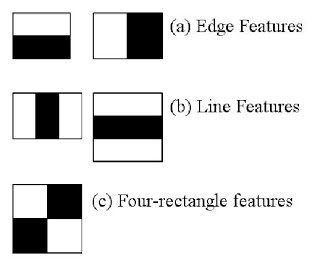
\includegraphics[width=0.5\linewidth]{figs/haar.jpg}
  \caption{Four kinds of HAAR feature rectangles \textnormal{\small }  }
  \label{fig:haar}
\end{figure}

\item \textbf{Integral Image}
The calculation of characteristic value of a feature is an important step in 
face detection. It has to be calculated for every possible pixel region in the given image. 
In order to efficiently determine the value, integral image of the given image is used. 
For any given pixel \emph{(x, y)}, the integral value is the sum of all the pixels above and to 
the left of \emph{(x, y)}, inclusive.
i,e., If \emph{v(x’, y’)} is the value of a pixel at \emph{(x’, y’)},  then the
Integral Sum is given by:

\vspace{0.1in}
\begin{center}
\begin{math}
    IS = \sum\limits_{x'\leqslant  x'y' \leqslant    y'} {v(x’, y’)}
\end{math}
\end{center}



\vspace{0.05in}
Now, the sum of any given region with corner integral pixels A, B, C, D is
\emph{Sum = D + A - B - C} as shown in Figure~\ref{fig:sum}.

\vspace{0.1in}
\begin{figure}[h]
  \centering
  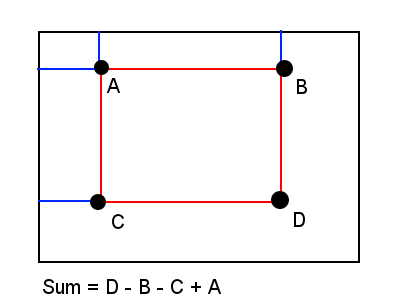
\includegraphics[width=0.5\linewidth]{figs/sum.png}
  \caption{Sum of a sub-window using Integral Image \textnormal{\small }  }
  \label{fig:sum}
\end{figure}

As shown in Figure~\ref{fig:example}, if we want to obtain the sum of 2x3 sub-window, 
integral image involves just 2 additions and 2 subtractions instead of 6 additions.

\begin{figure}[h]
  \centering 
  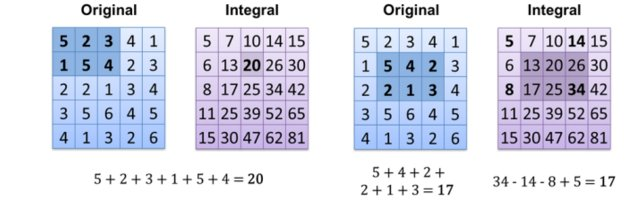
\includegraphics[width=\linewidth]{figs/example.jpg}
  \caption{Example of Integral Image calculation \textnormal{\small }  }
  \label{fig:example}
\end{figure}

\vspace{0.1in}
\item \textbf{Adaboost Algorithm} Adaboost or Adaptive Boosting is a machine learning algorithm 
where the output of weak classifiers is combined into a weighted sum that represents the output 
of a boosted (strong) classifier. This algorithm is used to combine features that cover facial 
characteristics to form a weak classifier. It then creates a string classifier using a group 
of weak classifiers. It further concatenates the strong classifiers to a cascade classifier.


\begin{figure*}[h]
  \centering
  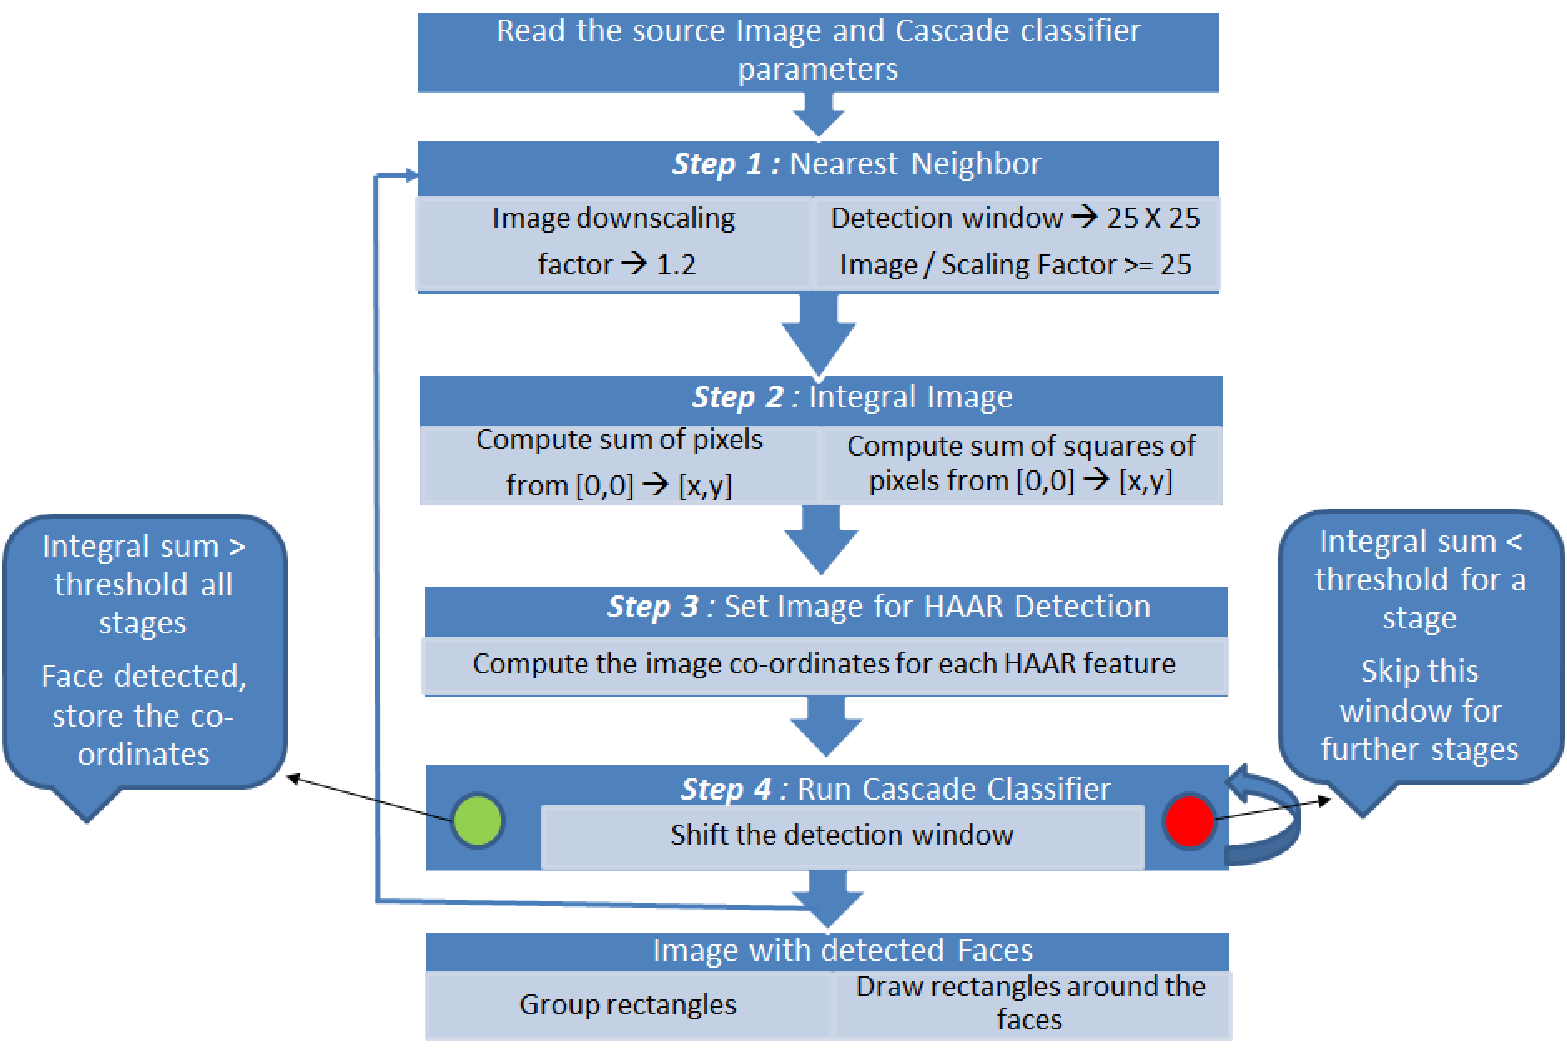
\includegraphics[width=0.75\linewidth]{figs/flow_crop.pdf}
  \caption{Face detection implementation flow }
  \label{fig:flow}
\end{figure*}



\vspace{0.1in}
\item \textbf{Cascade Classifier} A sub-window in the image that passes through the entire cascade 
classifier is detected as human face (Figure~\ref{fig:cascade}). In this project, we used 25 stages in cascade classifier.

\begin{figure}[h]
  \centering
  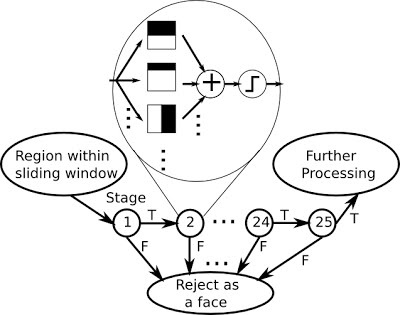
\includegraphics[width=0.8\linewidth]{figs/cascade.jpg}
  \caption{Cascade Classifier \textnormal{\small }  }
  \label{fig:cascade}
\end{figure}

\end{itemize}




\section{Our Implementation }\label{sec:impl}

In this project, we consider the sections in the algorithm that
can be parallelized, write kernels for each of them in CUDA
and offload them to be executed on GPU. The sections that
can be parallelized are explained below.

\vspace{0.1in}
\begin{itemize}

\item \textbf{Image Pyramid:}
We use fixed size (20x20) for each feature. But the face in the image can be of any scale. 
To make the face detection scale  invariant, we use pyramid of images that contains upscale and
downscale versions of the original image. Since each pixel can be processed separately, 
we intend to produce image pyramid on GPU. Example of an image pyramid is shown in Figure~\ref{fig:scale}.

\begin{figure}[h]
  \centering
  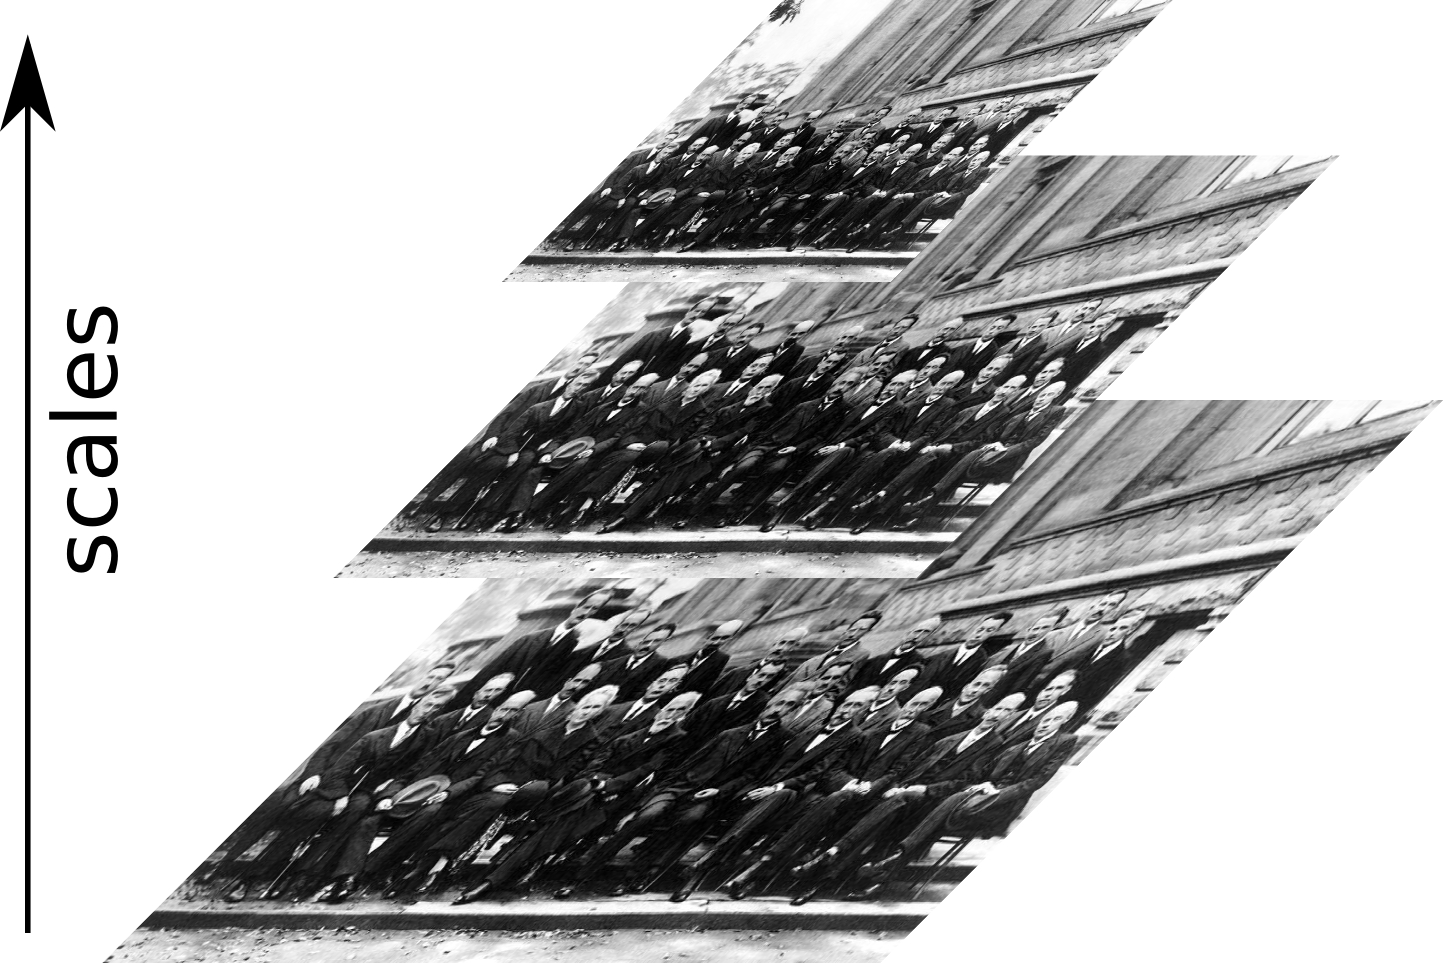
\includegraphics[width=0.65\linewidth]{figs/scale.jpg}
  \caption{Image Pyramid \textnormal{\small }  }
  \label{fig:scale}
\end{figure}


\item \textbf{Integral Image Calculation:}
Integral image calculation is essentially 2-dimensional inclusive scan. Since we have already done 
1-dimensional prefix scan on GPU and seen the benefits, we intend to determine integral image on 
similar lines.
To avoid data dependency of image integral calculation, we adopt the algorithm of first 
row integral and then column integral calculation.

\vspace{0.1in}
\item \textbf{Scan Window Processing:}
Since each 20x20 image sub-window has to pass through all the features, each thread in the GPU 
can perform parallely on a sub-window. But the design of cascade classifier is such that after 
each stage the doubtless non-face scan sub-windows are eliminated as much as possible. Hence we 
want to consider each stage separately and sequentially, may be execute each stage as a different kernel.
Figure~\ref{fig:scan} show th principle of using parallel scan windows.\fixme{Need a better pic for scan window} 

\begin{figure}[h]
  \centering
  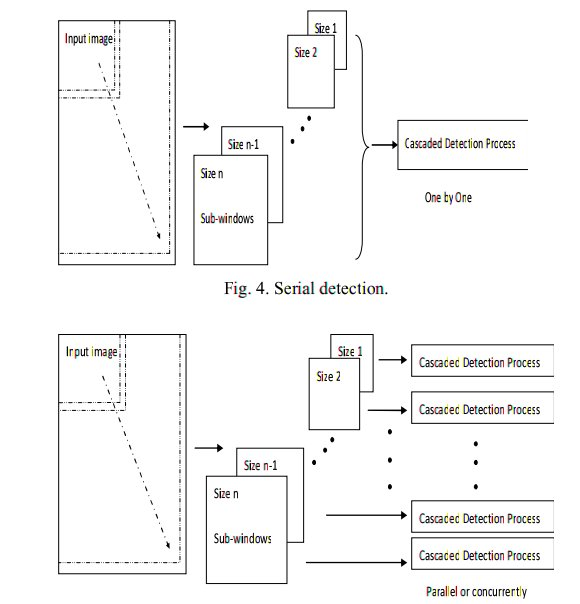
\includegraphics[width=\linewidth]{figs/scan.jpg}
  \caption{Parallel Scan Window Processing \textnormal{\small }  }
  \label{fig:scan}
\end{figure}



\end{itemize}


\section{Nearest Neighbor and Integral Image}\label{sec:nnii}

\fixme{Manoj holds the lock}


\section{HAAR Cascade Classifiers}\label{sec:haar}

\fixme{Sharmila holds the lock}


\section{Optimizations}\label{sec:optim}

\subsection{Optimizations in Nearest neighbor and Integral Image calculation}\label{sec:nn_optim}

\begin{itemize}

\item \textbf{Coalescence Of Global Memory Writes:}
To coalesce the reads \& writes to global memory the image matrix transpose was 
implemented in a tiled fashion in kernels 2 and 4 from Section~\ref{sec:impl nn II}. 
Figures~\ref{fig:naive} and ~\ref{fig:optim} show the naive 
and optimized implementation of the matrix transpose respectively from a memory 
access point of view. As the shared memory access are discrete\textit{(each word from a bank)}
and global memory accesses are coalesced(cacheline) by nature, we implemented the 
transpose as shown in figure 7. Once the data tile is brought into the shared memory, 
it was read column wise from it and then written row wise into global memory. 
Effectively, SM[Ty][Tx] is changed to SM[Tx][Ty]. 

\begin{figure}[h]
  \centering
  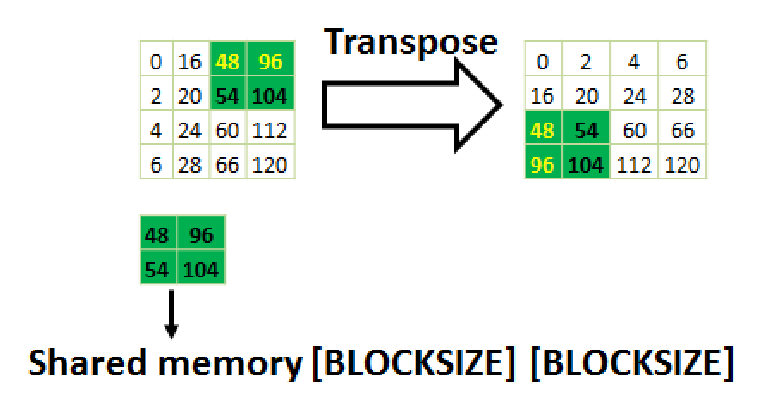
\includegraphics[width=\linewidth]{figs/nn_naive_crop.pdf}
  \caption{Naive Implementation of Matrix Transpose }
  \label{fig:naive}
\end{figure}

\begin{figure}[h]
  \centering
  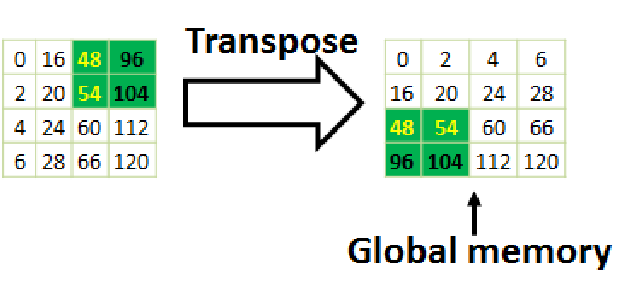
\includegraphics[width=0.9\linewidth]{figs/nn_optim_crop.pdf}
  \caption{Optimized Implementation of Matrix Transpose }
  \label{fig:optim}
\end{figure}

However, changing the reading pattern from a shared memory from 
row wise(Figure~\ref{fig:naive}) to column wise(Figure~\ref{fig:optim}), we need to make sure there 
aren’t any shared memory bank conflicts.

\vspace{0.1in}
\item \textbf{Elimination Of shared memory bank conflicts:}
SM bank conflicts occur when two or more threads in the same warp try to access the same memory bank. 
Let’s analyze the thread mapping to shared memory banks for this situation. Here in our implementation, 
we use a BLOCKSIZE of  16. Each (Tx, Ty) map to (Tx * 16 + Ty) \% 32  bank of an SM. (Tx, Ty) for (0, 0) \& (2, 0) 
\textit{(have global thread indices of 0 and 2 respectively, so belong to the same warp)} map to bank 0. 
So, we have a 2-way bank conflict introduced with the change in access pattern to SM. However, 
it is eliminated by making the (Tx * 16 + Ty) not a multiple of 32. 
Shared memory [BLOCKSIZE] [BLOCKSIZE + 1] was used to tackle this problem. 
Increasing the row width by 1 makes each mapping offset by 1 bank position.


\vspace{0.1in}
\item  \textbf{Use Extern To Declare Shared Memory:}
Hard coding the shared memory size tends to make it an inherent occupancy constraint 
though in practice it can be avoided. Instead, we can make it as extern, 
determine the size during runtime and pass it in kernel launch. Let’s analyze the 
RowScan kernel configuration to brief this situation.  

Kernel configuration: (w, h – width \& height of downscaled Image)
\begin{itemize}
    \item Threads per block = smallestpower2(w): Constraint from RowScan algorithm
    \item Blocks = h
    \item shared memory of 2 * (width of image + 1) (factor 2: One for integral sum \& other for square Integral sum).
\end{itemize}
At downscale of 256 X 256 image size (from source of 1024 X 1024 pixels), we launch a 1 dimensional 
grid of 256 blocks with 256 Threads Per Block (TPB). For this configuration, 6 blocks can be alive, 
giving a 100\% occupancy (1536 threads). Hardcoding the shared memory to that of max case 
of 1024 TPB (8kB SM)  decreases it to 5 blocks giving 84\% occupancy only. 

\end{itemize}


\subsection{Optimizations for Scan Window Processing}\label{sec:haar_optim}
\begin{itemize}

\item \textbf{Using Shared Memory:}
Information about the classifiers as mentioned in Section
\ref{sec:haar} are common to all the scan windows. Hence the first optimization 
is to bring the data related to classifiers. But since there are 2913 classifiers 
for the entire face detection process, it requires 209.836kB of storage for the data. 
But a maximum of 48kB shared memory is available. Hence we split the scan window processing 
into multiple kernels with n stages in each kernel that correspond to around 320 Haar classifiers. 
This requires 12 kernels with around 19kB of shared memory each.
Using Pinned Host Memory: When allocating memory on CPU for the data that needs to be transferred 
to GPU, there are two types of memory to choose from: \emph{Pinned} and \emph{Non-Pinned}. 
Pinned memory is not swapped out from the memory by the OS for any reason and hence provides 
improved transfer speeds. CUDA provides \emph{cudaMallocHost} API that can be used instead of 
usual \emph{malloc} to achieve this.

\vspace{0.1in}
\item \textbf{Using Fast Math:}
Our algorithm makes use of calculating standard deviation which is the square 
root of variance. If we make use of \emph{-use\_fast\_math} flag while compiling using \emph{nvcc}, 
we explicitly instruct GPU to use its Special Functional Unit to calculate square root. This provides 
lesser precision but at a greater speed. 

\vspace{0.1in}
\item \textbf{Not using restriction on maximum registers per thread:}
In our baseline implementation, we had 
restricted maximum register count per thread to 20 to increase occupancy. But scanning window 
kernel requires 28 registers. Because of the restriction there was spilling of registers that 
increased the execution time. Hence we removed the imposition and observed decreased execution 
time even though occupancy decreased. This showed occupancy is not always a measure of performance.

\vspace{0.1in}
\item \textbf{Using block divergence:}
In the baseline implementation, each thread continued execution up to 25 stages 
even if the scan window failed any previous stage. Rejecting a thread as early as possible leads to thread 
divergence that leads to under-utilization as in Figure~\ref{fig:tdiv}. But if all the threads in a block 
are rejected, block divergence occurs and the entire block will not be launched at all thus increasing 
performance as in Figure~\ref{fig:bdiv}. Since each kernel can consist of multiple stages, we reject a 
scan window at kernel-level granularity. Images that have one or two faces have only few scan windows that 
have face. Using this optimization, we have made the common case faster. Hence according to 
\emph{Amdahl’s law} we observe huge increase in performance. 

\end{itemize}
\begin{figure}[h]
  \centering 
  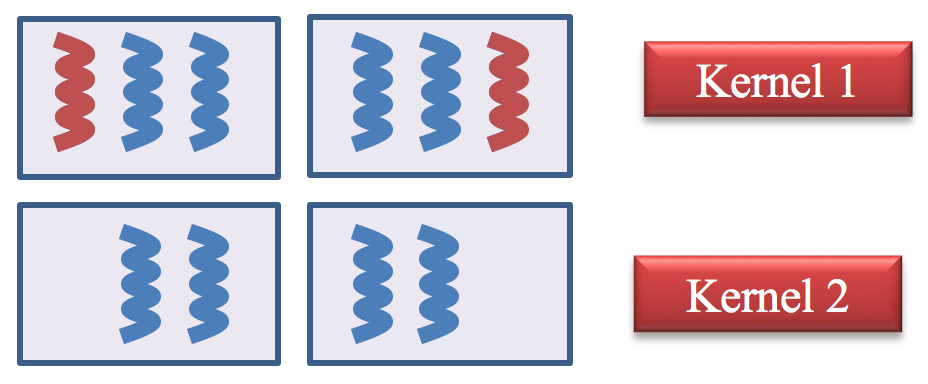
\includegraphics[width=\linewidth]{figs/thread_div.png}
  \caption{Example of Thread Divergence \textnormal{\small }  }
  \label{fig:tdiv}
\end{figure}


\begin{figure}[h]
  \centering 
  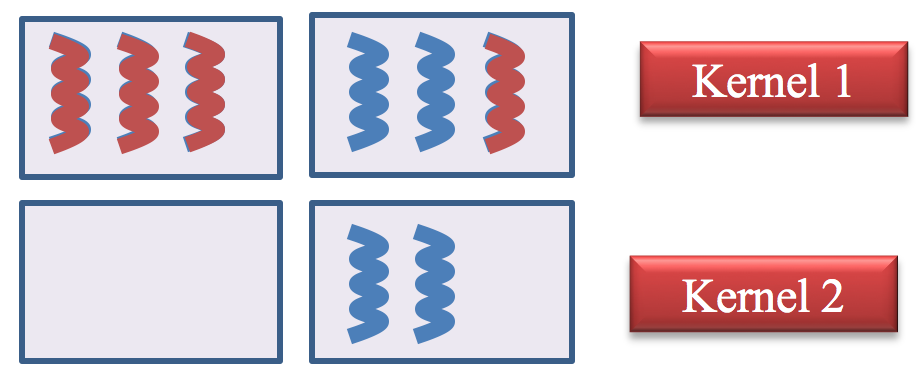
\includegraphics[width=\linewidth]{figs/block_div.png}
  \caption{Example of Block Divergence \textnormal{\small }  }
  \label{fig:bdiv}
\end{figure}



\section{Evaluation framework}\label{sec:eval}

\begin{table*}[th]
\centering
\scalebox{0.65}{
\begin{tabular}{|c|c|c|c|c|c|c|c|c|c|c|c|c|c|c|c|c|c|c|c|c|c|c|c|c|l|}
\hline
\textit{\textbf{Stage}}      & 1  & 2  & 3  & 4  & 5   & 6   & 7   & 8   & 9   & 10  & 11  & 12  & 13  & 14  & 15  & 16  & 17  & 18  & 19  & 20  & 21  & 22  & 23  & 24  & 25   \\ \hline 
\textit{\textbf{Classifiers}} & 9  & 16 & 27 & 32 & 52  & 53  & 62  & 72  & 83  & 91  & 99  & 115 & 127 & 135 & 136 & 137 & 159 & 155 & 169 & 196 & 197 & 181 & 199 & 211 & 200  \\ \hline
\textit{\textbf{Rectangles}} & 18 & 48 & 81 & 96 & 156 & 159 & 186 & 216 & 249 & 273 & 297 & 345 & 381 & 405 & 408 & 411 & 477 & 465 & 507 & 588 & 591 & 543 & 597 & 633 & 600  \\ \hline
\end{tabular}
}
\vspace{0.05in}
\caption{HAAR cascade classifier and its features}
\label{table:features}
\end{table*}

\begin{table*}[h]
    \centering
    \scalebox{0.75}{
    \begin{tabular}{|l|l|l|l|l|l|l|}
        \hline
        \textbf{Kernel}                   & \multicolumn{2}{l|}{\textbf{Registers}}    & \textbf{Shared memory (KB)} & \textbf{Constant Memory (Bytes)} & \multicolumn{2}{l|}{\textbf{Occupancy (\%)}} \\ \hline
        \textbf{}                         & \textbf{With Maxreg} & \textbf{w/o Maxreg} & \textbf{}                   & \textbf{}                        & \textbf{With Maxreg}  & \textbf{w/o Maxreg}  \\ \hline
        \textbf{NN + RowScan}             & 18                   & 18                  & 8.2                         & 88                               & 100                   & 100                  \\ \hline
        \textbf{Transpose 1}              & 12                   & 12                  & 2.1                         & 60                               & 100                   & 100                  \\ \hline
        \textbf{RowScan Only}             & 17                   & 18                  & 8.2                         & 72                               & 100                   & 66.67                \\ \hline
        \textbf{Transpose 2}              & 12                   & 12                  & 2.1                         & 60                               & 100                   & 100                  \\ \hline
        \textbf{HAAR Cascade Classifiers} & 20                   & 28                  & 19.5                        & 156                              & 66.67                 & 66.67                \\ \hline
    \end{tabular}
    }
    \vspace{0.05in}
    \caption{Registers, Shared Memory, Constant Memory and Occupancy for all the kernels}
    \label{table:util}
\end{table*}




For this project, we evaluate the performance and resource utilization 
of face detection algorithm on GPGPU implementation with that of a CPU. 
We are not considering the
cascade classifier training part and are directly taking a CPU version of
previously trained classifier. Offline training of the classifier network
for different images on GPU will be implemented as part of our future work.
For now, the trained cascade classifier consists of 
number of stages needed for face detection, HAAR features needed in each
stage, the rectangles of each feature, threshold values for each stage and classifier.

\begin{table}[h]
    \centering
    \scalebox{0.85}{
    \begin{tabular}{|l|l|}
        \hline
        \textbf{CUDA runtime version}         & 7000                  \\ \hline
        \textbf{CUDA driver version}          & 7050                  \\ \hline
        \textbf{}                             &                       \\ \hline
        \textbf{Device Name}                  & GeForce GTX 480       \\ \hline
        \textbf{Compute Capability}           & 2.0                   \\ \hline
        \textbf{Global Memory (MB}            & 1535                  \\ \hline
        \textbf{Total Const Memory (KB}       & 64                    \\ \hline
        \textbf{Shared Memory per Block (KB)} & 48                    \\ \hline
        \textbf{Shared Memory per SM (KB)}    & 48                    \\ \hline
        \textbf{L2 Cache Size (KB)}           & 768                   \\ \hline
        \textbf{Registers per Block}          & 32768                 \\ \hline
        \textbf{Registers per SM}             & 32768                 \\ \hline
        \textbf{SM Count}                     & 15                    \\ \hline
        \textbf{max threads per SM}           & 1536                  \\ \hline
        \textbf{Max threads per block}        & 1024                  \\ \hline
        \textbf{Max thread dims}              & (1024, 1024, 64)      \\ \hline
        \textbf{Max grid size}                & (65535, 65535, 65535) \\ \hline
        \textbf{Num copy engines}             & 1                     \\ \hline
    \end{tabular}
    }
    \vspace{0.05in}
    \caption{Arch. details of the GPU card used}
    \label{table:device}
\end{table}

\vspace{-0.1in}
\begin{table}[h]
    \centering
    \scalebox{0.85}{
    \begin{tabular}{|l|l|}
        \hline
        \textbf{Architecture}        & x86\_64                            \\ \hline
        \textbf{CPU(s)}              & 16                                 \\ \hline
        \textbf{On-line CPU(s) list} & 0-15                               \\ \hline
        \textbf{Thread(s) per core}  & 2                                  \\ \hline
        \textbf{Core(s) per socket}  & 4                                  \\ \hline
        \textbf{Socket(s)}           & 2                                  \\ \hline
        \textbf{Model name:}         & Intel Xeon(R) CPU E5520 @ 2.27 GHz \\ \hline
        \textbf{CPU MHz}             & 1600                               \\ \hline
        \textbf{L1d cache (KB)}      & 32                                 \\ \hline
        \textbf{L1i cache (32KB)}    & 32                                 \\ \hline
        \textbf{L2 cache (KB)}       & 256                                \\ \hline
        \textbf{L3 cache (MB)}       & 8                                  \\ \hline
    \end{tabular}
    }
    \vspace{0.05in}
    \caption{Arch. details of the CPU used}
    \label{table:cpu}
\end{table}

\vspace{0.3in}
Table~\ref{table:features} gives an overview and information of the total number of stages
used, number of filers/classifiers in each stage and rectangle features used in each stage.
Apart form that, each rectangle has a weight associated with it, each classifier has a threshold value and each stage
also has a threshold value. These threshold values are used at each step of scan window processing
and would determine whether the face is present in the downsampled image. 



\paragraph{}
We compared the GPU exclusive time (kernel time),
inclusive time (kernel + CPU to GPU copy time) with the CPU execution time 
for face detection in an image.
As mentioned in Section~\ref{sec:impl}, we have parallelized three different
portions in the algorithm and in Section~\ref{sec:results} we analyze the results of each of this kernel.
We evaluated our face detection implementation on an NVIDIA GTX 480 GPU card with 15 SMs and 1.5GB global memory.
Table~\ref{table:device} gives the architecture details of the device on which we evaluated the kernels. For comparison with CPU, 
we used 16 core Intel Xeon CPU, but since the Viola Jones code was a single threaded code, the comparison is only with
1 core of CPU. Table~\ref{table:cpu} gives the architecture details of the CPU used for comparison. 
We also use all the optimizations applied for the kernels (Section~\ref{sec:optim}) and show the
results for these optimizations. 

We considered different image sizes during our evaluation and our kernels can fit and detect
the largest  image of size 1024 x 1024. For all our further performance analysis, we use this the image size of 1024 x 1024 
and it involves 21 iterations of downsampling until it reaches the minimum size of 25 x 25.

For profiling and bottleneck analysis, we used
NVIDIA Visual Profiler~\cite{rosen2013visual} and then take corresponding decisions for performance boost. CUDA profilers also helped us to gain an understanding 
of the kernel occupancy and their shared memory usage.
We use CUDA events~\cite{wilt2013cuda} for timing analysis of GPGPU (both exclusive and inclusive) and
CPU execution.  


 
\section{Results}\label{sec:results}

In this section, we overview the performance results and the resource
utilization all the kernels implemented on GPU for face detection. 
Although, occupancy is not a direct measure of performance, it is important 
to have full occupancy for the GPU SMs. Based on the utilization analysis done for all the kernels,

Table~\ref{table:util} shows the occupancy of each of the kernels. This includes the registers, 
shared memory and constant memory used for the kernels. As discussed in Section~\ref{sec:haar_optim}, 
relaxing the maximum registers used by thread is an optimization. We apply this optimization and check for the 
occupancy of each kernel. 
However, this constraint can be relaxed only if all the threads in the thread block can accommodated with that register usage.
In our case, relaxing this constraint did not put a constraint on the threads that can be launched with each kernel.
We see that for \emph{RowScan Only} kernel the occupancy reduces due to this relaxation. However, the results of that kernel
show that it did not impact for the performance. 


\begin{figure*}
  \centering
  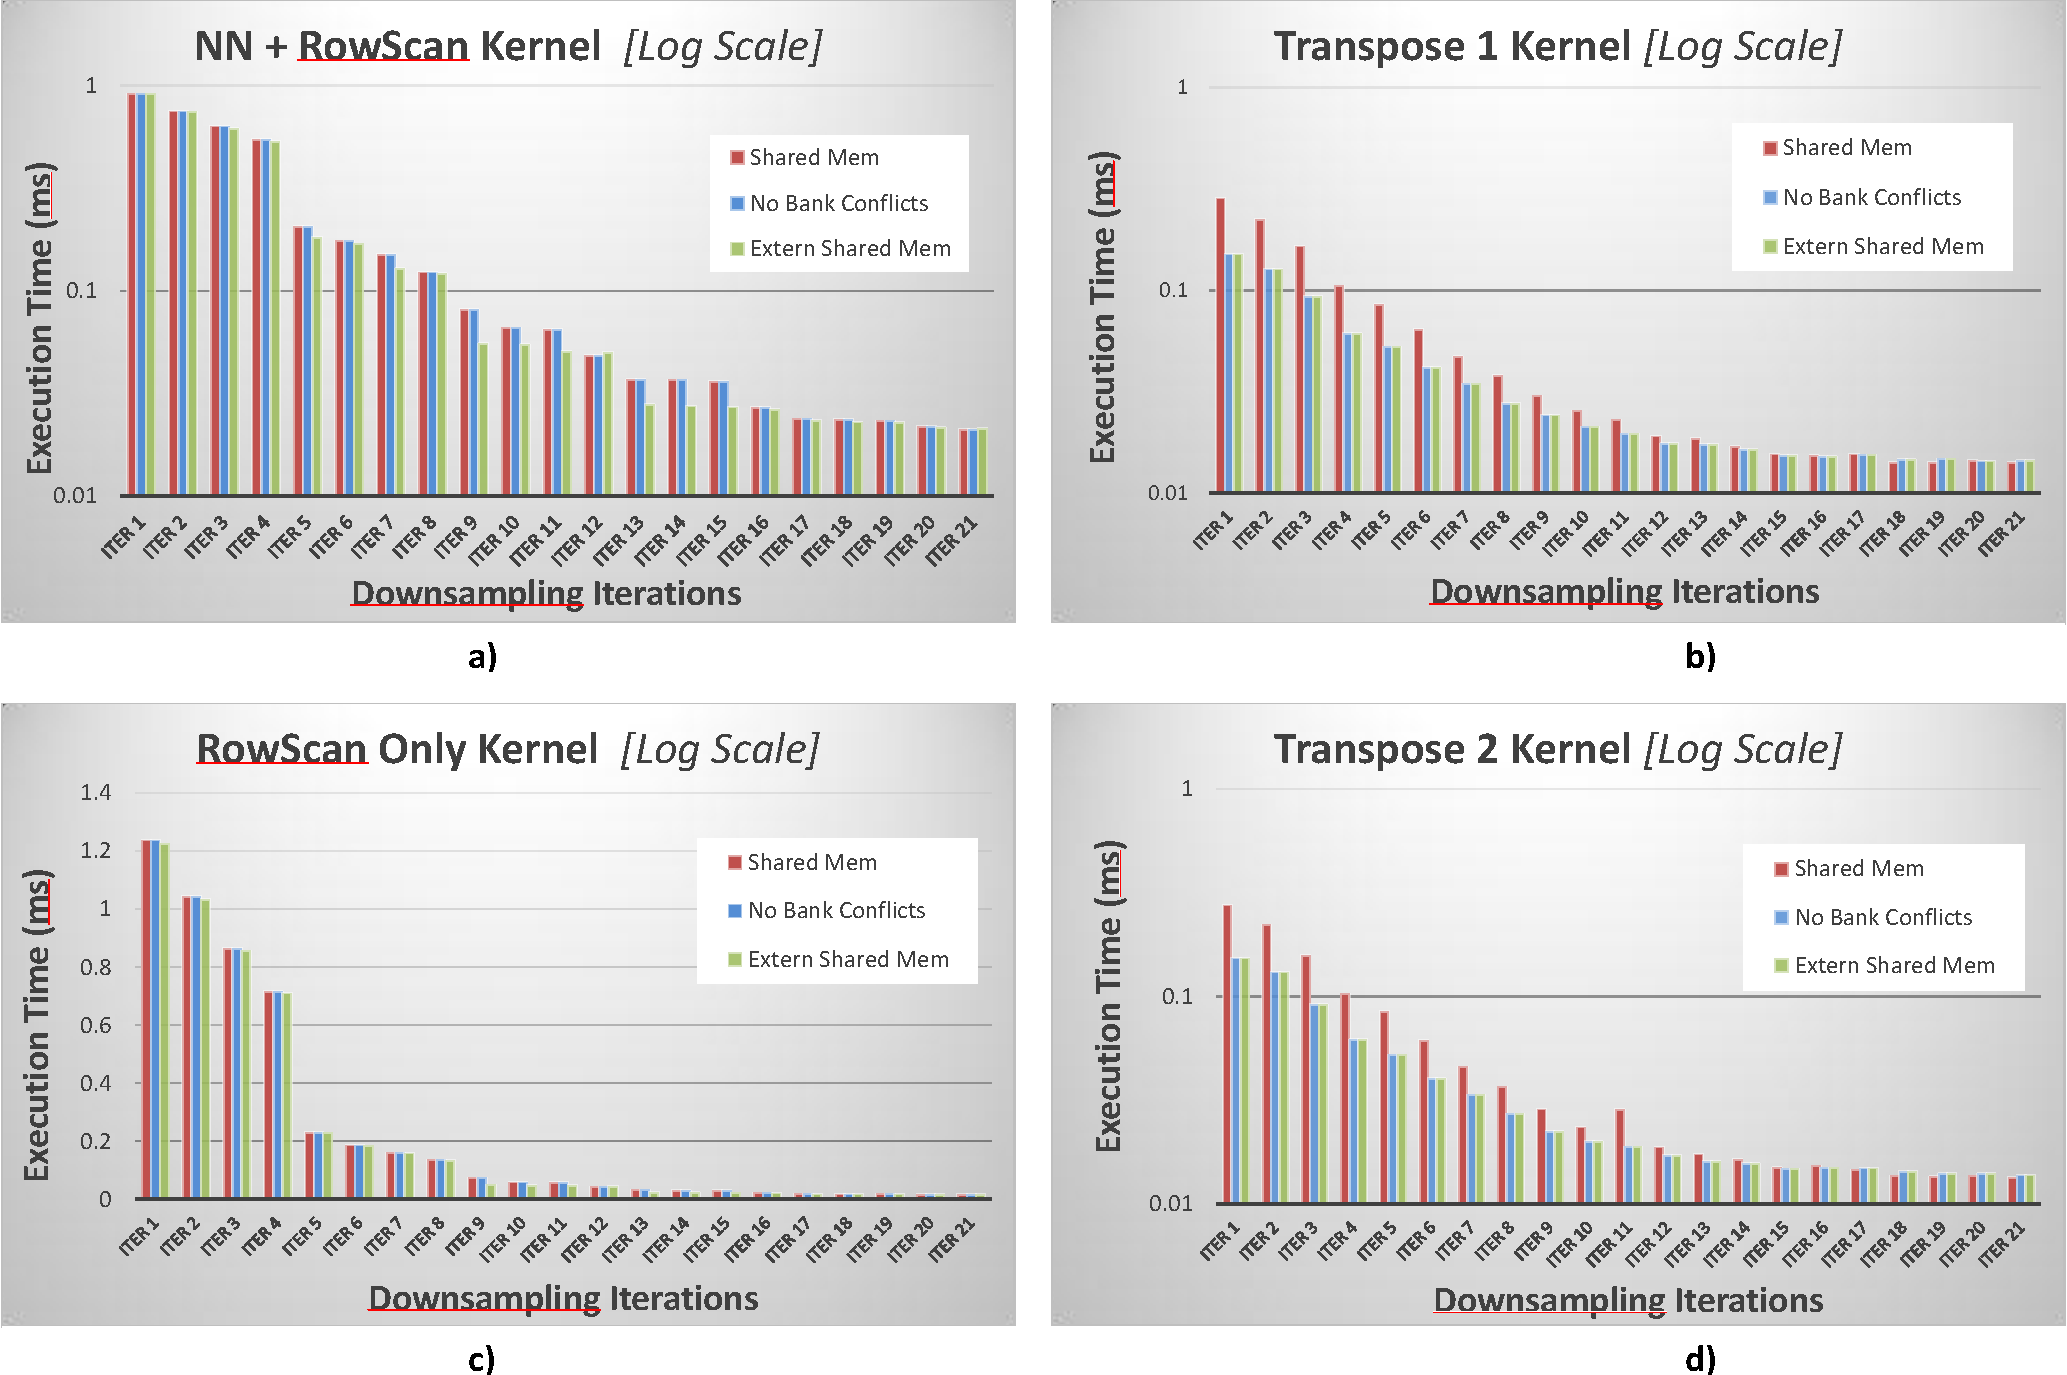
\includegraphics[width=\linewidth]{figs/nn_ii_kernels_crop.pdf}
  \caption{Performance of NN and II kernels; a) NN + RowScan; b) Transpose 1; c) RowScan Only; d) Transpose 2}
  \label{fig:nn_ii_kernels}
\end{figure*}

\vspace{0.2in}
\begin{figure*}[h]
  \centering
  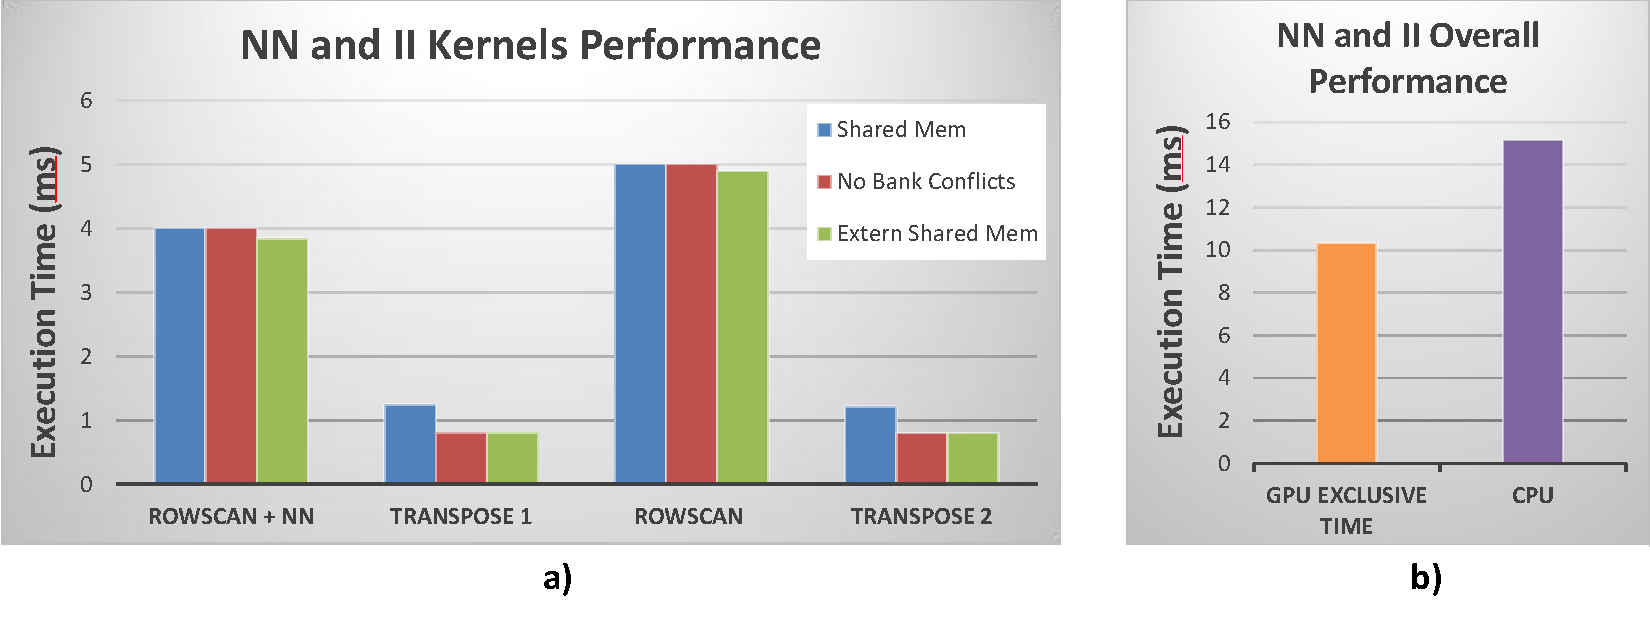
\includegraphics[width=0.9\linewidth]{figs/nn_ii_overall_crop.pdf}
  \caption{a) NN and II kernels performance for all optimizations; b) Overall NN + II performance over CPU}
  \label{fig:nn_ii_overall}
\end{figure*}

\subsection{Performance of Nearest Neighbor and Integral Image Kernels}
Figure~\ref{fig:nn_ii_kernels} shows the performance of individual kernels of NN and II stage.
We apply the 3 optimizations discussed in Section~\ref{sec:nn_optim} here. Since, NN and II kernels 
contributed to only 3\% of the overall parallelization scope, we directly implemented the Shared memory version of the kernels
and that act as the baseline for NN and II kernels. When we applied the \emph{No bank conflicts} optimization, only the \emph{Transpose 1}
and \emph{Transpose 2} kernel showed the benefit in reducing the execution time. This is because, transpose kernels are tiled implementations, 
and are initially brought from global memory to shared memory (by reading row wise) and are then read column wise from shared memory. While reading column wise, 
you encounter bank conflicts and to reduce this, we applied \emph{No bank conflicts} optimization. \emph{NN + RowScan} and \emph{RowScan} kernels do not show 
any improvement as they do not suffer from bank conflicts. 

Second optimization we applied was the external declaration of shared memory
to reduce the shared memory constraint on thread blocks and thus performance. Here in this case,
\emph{NN + RowScan} and \emph{RowScan} kernels show benefit after iteration 9 at which the size of the 
downsampled image is 256 x 256. At this scale of image, external declaring the shared memory reduced the 
pressure on shared memory usage and more thread blocks could be launched. However, \emph{Transpose 1 } and 
\emph{Transpose 2} kernels do not show any benefit as they are tiled implementation and have fixed 16 x 16 thread block
size across all the downsampled image sizes. 


\begin{figure*}[h]
  \centering
  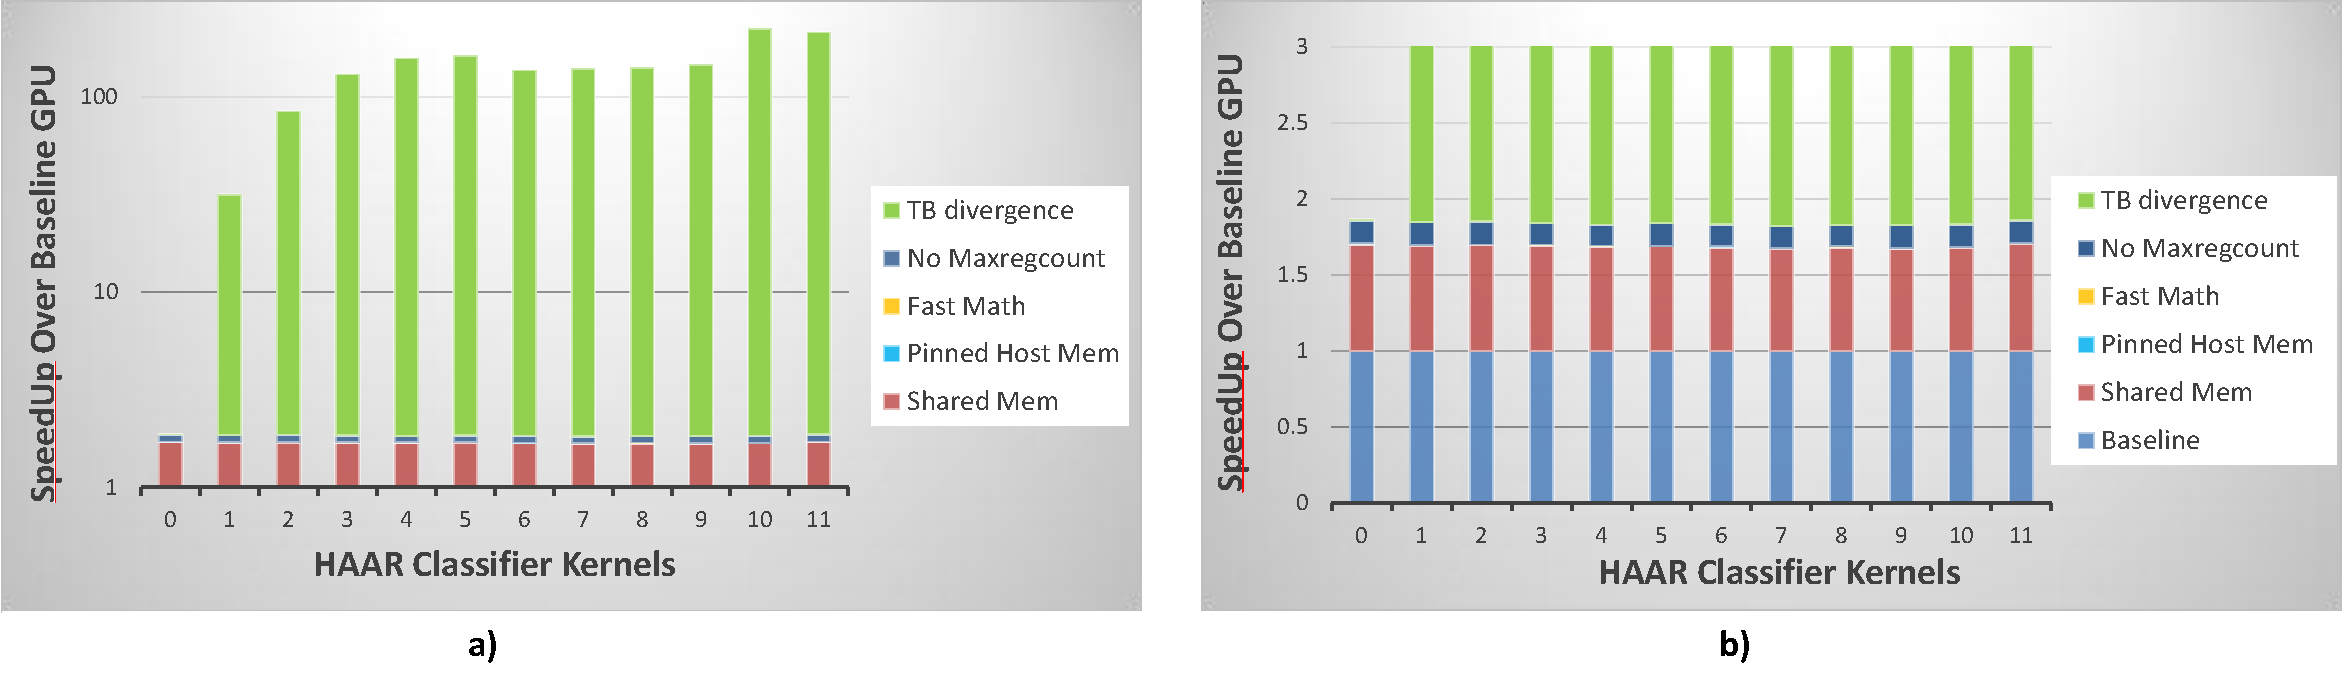
\includegraphics[width=\linewidth]{figs/haar_kernels_crop.pdf}
  \caption{a) HAAR kernels performance; b) Speedup with baseline GPU implementation and magnified version of a)}
  \label{fig:haar_kernels}
\end{figure*}


\begin{figure*}[h]
  \centering
  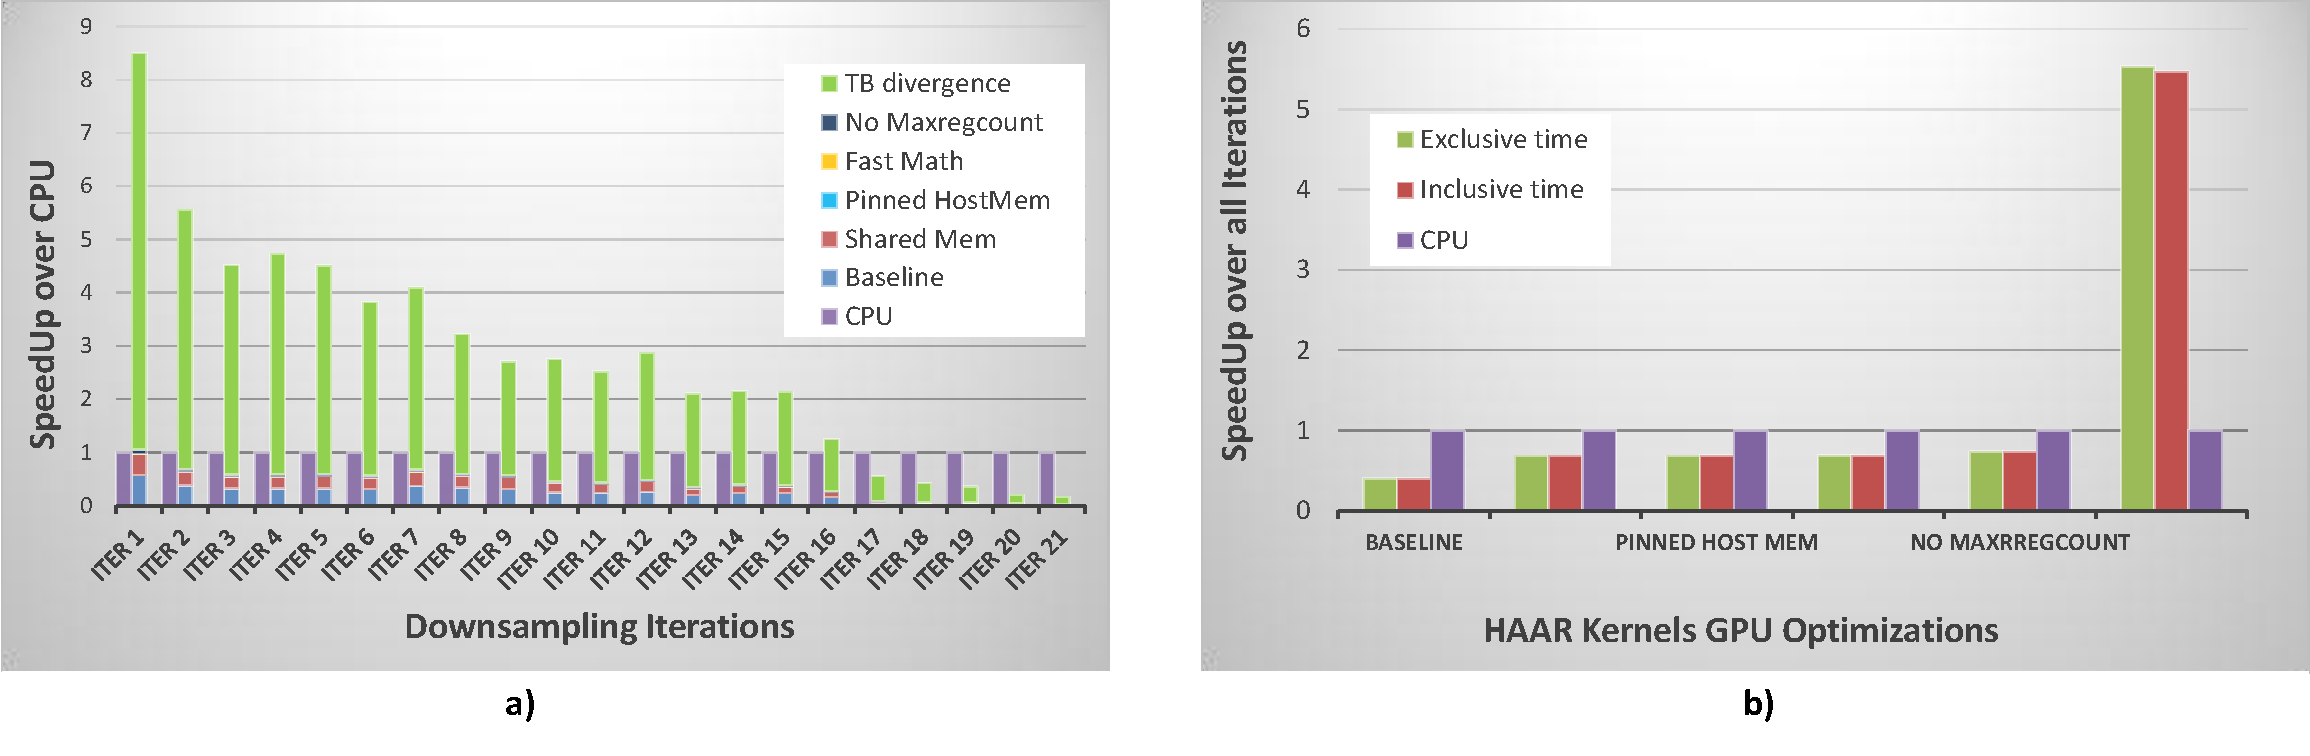
\includegraphics[width=\linewidth]{figs/haar_overall_crop.pdf}
  \caption{a)Performance of HAAR kernels over 21 iterations of 1024 x 1024 image face detection; b) HAAR kernels speedup over CPU for all the iterations}
  \label{fig:haar_overall}
\end{figure*}


\paragraph{}
Figure~\ref{fig:nn_ii_overall} \color{red}{a)} \color{black}{shows} the performance of all 4 NN and II kernels with the optimizations
applied. In overall, we see that \emph{NN + RowScan}, \emph{RowScan} kernels benefit from \emph{extern shared memory} declaration optimization 
and \emph{Transpose 1}, \emph{Transpose 2} kernels take significant benefit from \emph{No bank conflicts} optimization.

Figure~\ref{fig:nn_ii_overall} \color{red}{b)} \color{black}{shows} the combined kernels speedup on GPU over CPU. Here, we just consider the GPU exclusive time as these
kernels don't have any data copying. In overall, we see around \textbf{1.46x} speedup for NN and II kernels over CPU. 
We take the these best performing NN and II kernels for all future evaluations with HAAR classifier kernels.


\subsection{Performance of HAAR Classifier Kernels}
This section overviews the performance of HAAR classifier kernels which
has 97\% of parallelization scope for our face detection implementation.
Figure~\ref{fig:haar_kernels} \color{red}{a)} \color{black}{shows} the performance of 12 HAAR kernels for the image 1024 x 1024 (1 iteration) with optimizations 
detailed in Section~\ref{sec:haar_optim}.
Figure~\ref{fig:haar_kernels} \color{red}{b)} \color{black}{is} the magnified version showing the lower level speedup is detail. The overall speedup of each kernel
is mentioned in the top.
We see that the \emph{shared memory} gives around 1.7x benefit over the baseline GPU implementation. \emph{Pinned host memory} gives almost no benefit
due to the fact that there is very less copying involved in between the kernels. \emph{Fast math} library optimization also gives very negligent performance
as the HAAR kernel involves only 1 \textit{sqrt} function. By removing the maximum registers constraint (\emph{no maxreg} optimization), we get around
1.8x performance benefit over baseline. Finally, the biggest performance boost we get is from the \emph{thread block divergence}, which ranges from 29x to 220x speedup.
Kernel 1 sees no benefit because most of the heavy lifting is done here and it sees no thread block divergence. Whereas, all the other kernels see divergence and get benefited from that.


Figure~\ref{fig:haar_overall} \color{red}{a)} \color{black}{shows} the performance of combined 12 HAAR kernels performance for all the 21 iterations
of the 1024 x 1024 image face detection with all the optimizations explained above. Here, the baseline is CPU and we compare the performance of
all 21 iterations with single threaded performance of CPU. We see similar trend of performance benefit added from the optimizations and we get speedup upto 8.4x
over CPU (this includes the copy time between each kernel). However, it is interesting to see that after iteration 17 GPU has worse performance than the CPU. This is because of the
reason that, from that stages the kernel launch and thread creation overhead if more than the benefit you can get from parallelization. This is an indicator that for smaller images and
when there is low data or thread level parallelism available GPU performs worse than CPU.
Figure~\ref{fig:haar_overall} \color{red}{b)} \color{black}{shows} the combined performance of the entire scanning window stage (12 HAAR kernels with all 21 iterations) with each optimization added. 
We see that thread block divergence gives us the largest benefit of speedup upto \textbf{5.47x} (inclusive time) compared to CPU. We use this optimized kernel for the final face detection speedup comparison.


\subsection{Face Detection Speedup}
We now explain the overall speedup we achieved for the entire face detection algorithm implemented on GPU.
This includes the optimized version of NN + II kernels and optimized version of the HAAR kernel.

\vspace{-0.1in}
\begin{figure}[h]
  \centering
  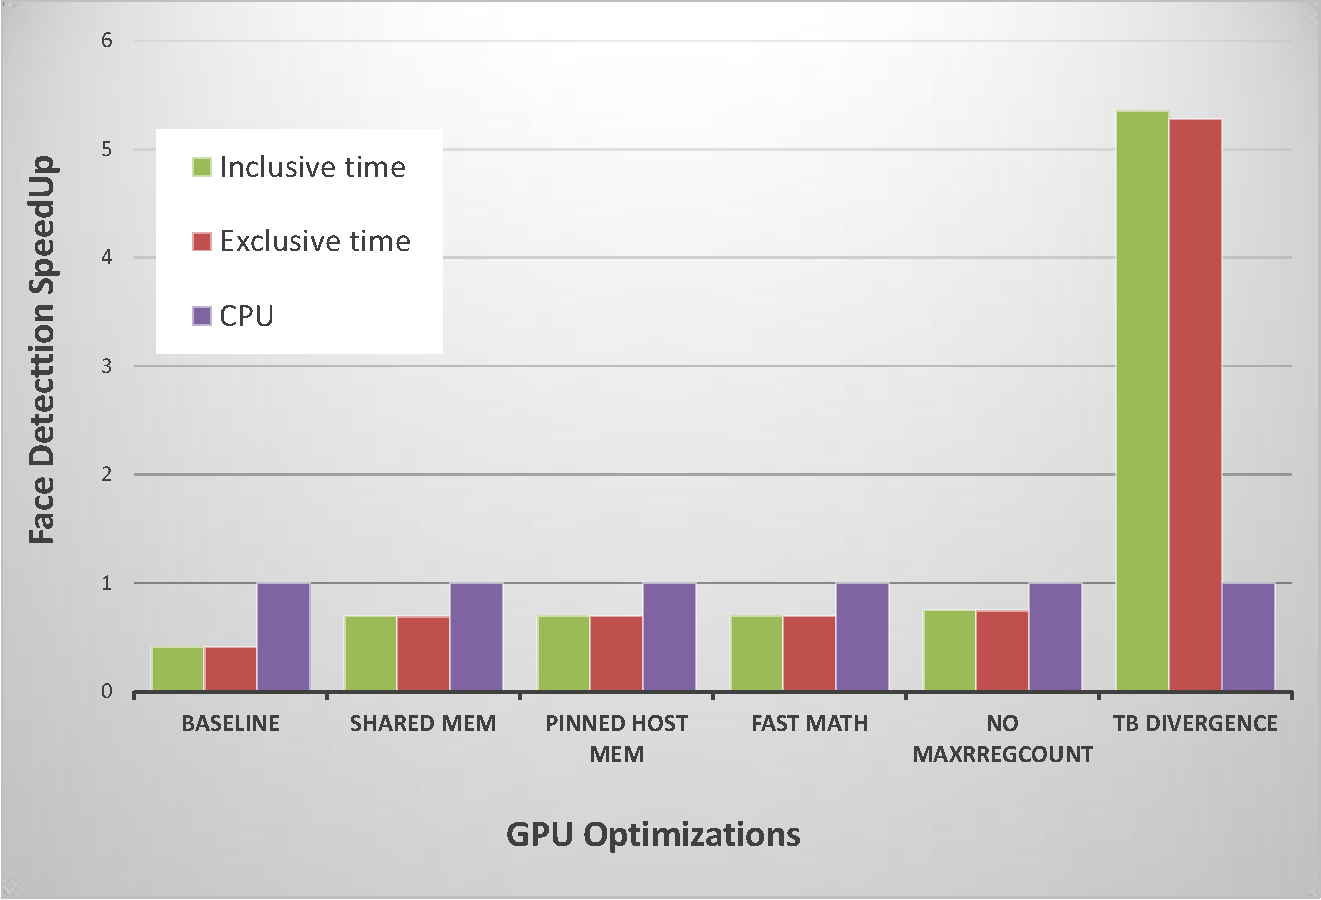
\includegraphics[width=\linewidth]{figs/gpu_overall_crop.pdf}
  \caption{Overall face detection speedup on GPU}
  \label{fig:gpu_overall}
\end{figure}

\vspace{-0.1in}
Figure~\ref{fig:gpu_overall} shows the overall face detection speedup of our implementation 
on GPU. We get a speedup upto \textbf{5.35x} overall over CPU and this includes the inclusive time of copying the
original source image to GPU. We believe this is a good speedup given the amount of serial dependency among HAAR 
classifier kernels. We believe that if parallel scan window processing could be implemented an extra 2-3x speedup can easily be achieved.


\subsection{Scalability and Detection Accuracy}
Figure~\ref{fig:img_sizes} shows GPU face detection speedup over CPU with increasing image sizes. 
As seen in previous results, GPU's parallelization benefit kicks in only after 128 x 128 image size as there
is abundant amount of data and thread level parallelism. As the image size increases GPU easily outperforms CPU and we see
upto 535x speedup with 1024 x 1024 image size. We expect that the speedup increases linearly as we scale up the image.



\begin{figure}[h]
  \centering
  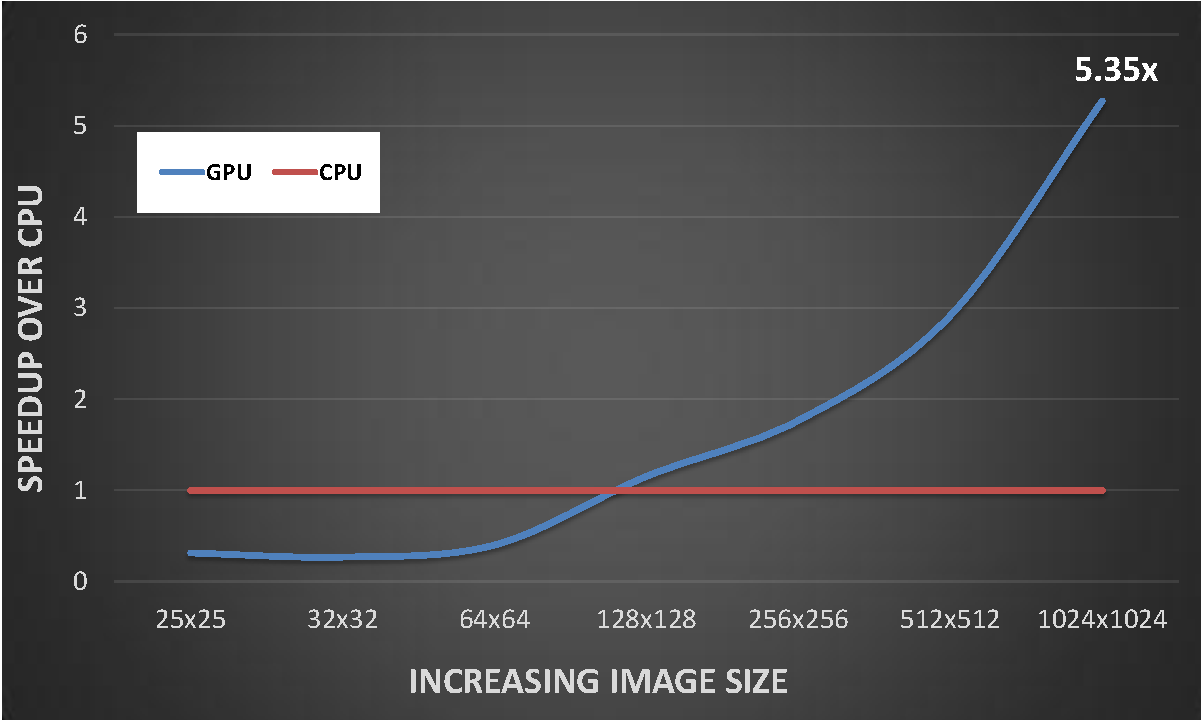
\includegraphics[width=\linewidth]{figs/image_size_crop.pdf}
  \caption{GPU speedup with varying image sizes}
  \vspace{0.05in}
  \label{fig:img_sizes}
\end{figure}

\begin{table}[]
    \centering
    \scalebox{0.65}{
        \begin{tabular}{|c|c|c|c|c|c|l|c|}
        \hline
        \textbf{Number of Faces}     & \textit{1} & \textit{2} & \textit{4} & \textit{8} & \textit{16} & 32    & \textit{Average Detection Rate (\%)} \\ \hline
        \textbf{Detection Rate (\%)} & 100        & 100        & 100        & 87.5       & 100         & 93.75 & \textbf{96.875}                      \\ \hline
        \end{tabular}
        }
        \vspace{0.1in}
        \caption{Face Detection Accuracy on GPU}
        \label{table:acur}
\end{table}


We also performed a small experiment of the algorithm accuracy. Although this is an algorithmic perspective
and not the implementation outcome, we  wanted to see how well the Viola Jones algorithm performs on GPU in detecting faces. 
Table~\ref{table:acur} shows the detection accuracy for different number of faces in the image. With random selection of images and
number of faces, we see upto 96.875\% accuracy in detecting faces. Figure~\ref{fig:detect} shows some example faces detected and as the accuracy test
confirm, one of the faces did not get detected in the test. This could be because of tilted face, or some of the features not present in the classifier filters.
But still given the simple classifier information, face detection can be easily be extended on GPU for better speedups and with more robust face detection algorithms
we expect to get better speedups and detection rate. 

\begin{figure}[h]
  \centering
  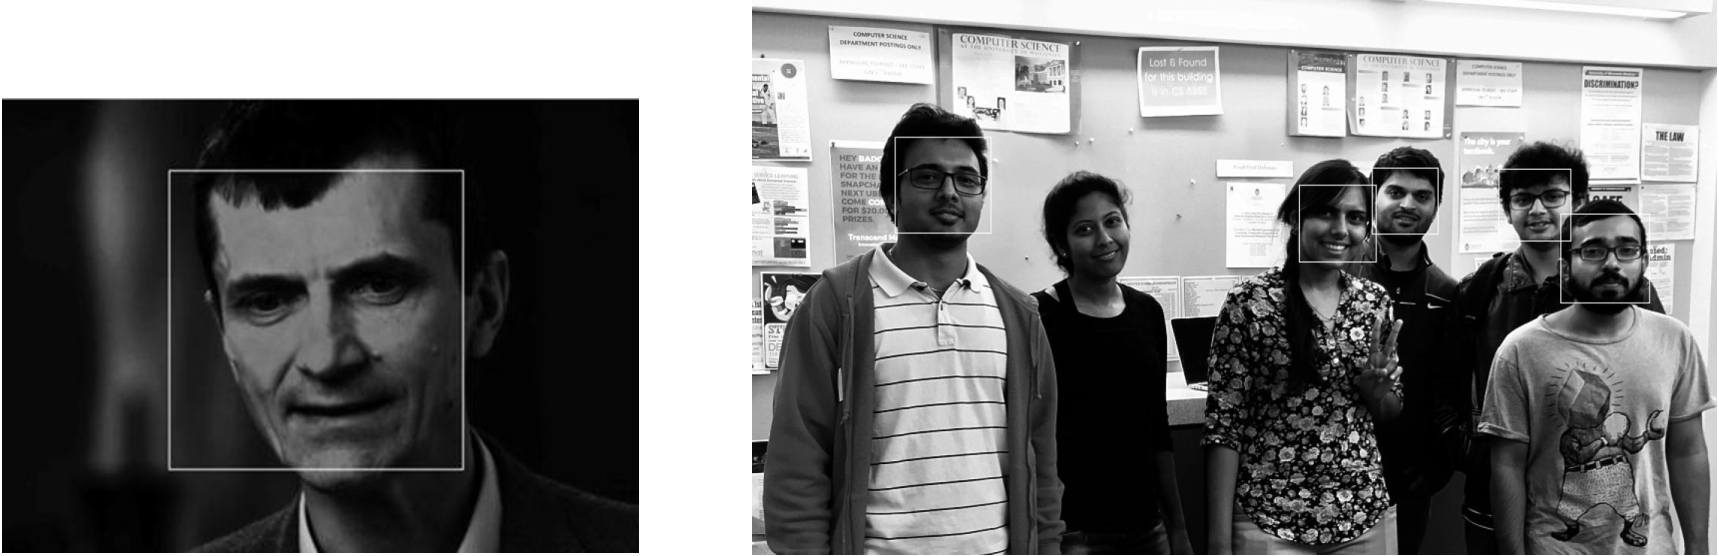
\includegraphics[width=\linewidth]{figs/face_detected_crop.pdf}
  \caption{Examples of faces detected on GPU}
  \label{fig:detect}
\end{figure}




\section{Related Work}\label{sec:related}


\section{Limitations and Future Work}\label{sec:future}

\fixme{Vinay holds the lock}

\section{Conclusion}i\label{sec:conc}

\fixme{Vinay holds the lock}

%
\bstctlcite{bstctl:etal, bstctl:nodash, bstctl:simpurl}
\bibliographystyle{IEEEtranS}
\bibliography{main}

\end{document}
